\documentclass[a4paper,11pt]{extarticle}

\usepackage{cursoice}

% ----------------------------------------------
% custom title
% ----------------------------------------------
\makeatletter
\renewcommand*{\maketitle}{%
\noindent
\begin{minipage}{0.2\textwidth}
	
\includegraphics[width=\textwidth]{img/logo_dte.png}
\end{minipage}
\hspace{1em}
\begin{minipage}{0.56\textwidth}
	
\begin{tikzpicture}
	\node[rectangle,rounded corners=6pt,inner sep=10pt,fill=blue!50!black,text width= 0.95\textwidth] {\color{white} {\Huge \@title} \\ {\Large}};
	\end{tikzpicture}
\end{minipage}
\hspace{1em}
\begin{minipage}{0.1\textwidth}
	
\includegraphics[width=\textwidth]{img/logo_teleco_2.png}
\end{minipage}
\hfill
\bigskip\bigskip
}%
\makeatother
% ------------------------------------------------

% ------------------------------------------------
% custom section
% ------------------------------------------------
\usepackage[explicit]{titlesec}
\newcommand*\sectionlabel{}
\titleformat{\section}
  {\gdef\sectionlabel{}
   \normalfont\sffamily\Large\bfseries\scshape}
  {\gdef\sectionlabel{\thesection\ }}{0pt}
  {
\noindent
\begin{tikzpicture}
\node[rectangle,rounded corners=3pt,inner sep=4pt,fill=blue!50!black,text width= 0.95\columnwidth] {\color{white}\sectionlabel#1};
\end{tikzpicture}
  }
\titlespacing*{\section}{0pt}{15pt}{2pt}
% -----------------------------------------------

% -----------------------------------------------
% custom footer
% -----------------------------------------------
\usepackage{fancyhdr}
\makeatletter
\pagestyle{fancy}
\fancyhead{}
\fancyfoot[C]{\footnotesize  \@date\ \ \@author}
\renewcommand{\headrulewidth}{0pt}
\renewcommand{\footrulewidth}{0pt}
\makeatother
% -----------------------------------------------


\title{Programación concurrente en Rust}
\author{Santiago Higuera. Universidad Politécnica de Madrid}
\date{\today}


\newcommand{\raya}{
	\vspace{0.5em}
	{\centering \rule{10cm}{0.1mm} \par}
	\vspace{0.5em}
}

\begin{document}

\maketitle

{\centering \footnotesize \textbf{\color{red}(Versión de fecha  \today)} \par}


%\setcounter{tocdepth}{1}
%\vspace*{3em}
%\tableofcontents

%\vfill
\begin{Resumen}

Apuntes sobre programación concurrente iniciados con la lectura del libro <<Rust Atomics and Locks. Low-Level Concurrency in Practice>>, de Mara Bos \citep{bosRustAtomicsLocks2023}. Este libro se puede acceder en línea a través del siguiente enlace:

{\centering \url{https://marabos.nl/atomics/} \par}

\smallskip

Además, es interesante el blog que mantiene la autora en:

{\centering \url{https://blog.m-ou.se/} \par}

\end{Resumen}

\section{Introducción}
Es difícil definir el concepto de \textit{Programación Funcional}. Se considera que la programación funcional está incluida en el paradigma de la \textit{programación declarativa}. En la programación declarativa, los lenguajes se centran en describir qué quieren hacer, en vez de detallar cómo quieren hacerlo, como sucede en los lenguajes imperativos.

Se considera que la programación funcional está basada en el \textit{cálculo lambda},  un sistema formal desarrollado en los años 1930 para investigar la naturaleza de las funciones, la naturaleza de la computabilidad y su relación con la recursión. 

En la programación funcional se pone especial énfasis en la utilización de \textit{funciones puras}. Una \textit{función pura} es aquella cuyo resultado solo depende del valor de los parámetros de entrada y que no da lugar a ningún efecto secundario. Siempre que se llame a la función con el mismo valor para los parámetros, se obtendrá el mismo resultado. Serían análogas a las funciones matemáticas.

Se entiende por \textit{efecto secundario} cualquier acción del programa que no sea un cálculo. Por ejemplo, modificar el estado de una variable, mostrar un mensaje en una pantalla o enviar un correo electrónico serían ejemplos de efectos secundarios.

Otro de los elementos fundamentales en cualquier lenguaje funcional es la consideración de las funciones como elementos de primera clase, esto es, poder utilizar las funciones como cualquier otro tipo de datos, poderlas asignar a una variable, poder pasarlas como parámetros a otras funciones o poder recibirlas como resultado de las mismas. A día de hoy, son muchos los lenguajes que han incorporado esta característica en sus funciones. 

En programación funcional es habitual utilizar un tipo especial de funciones denominadas \textit{closures}. Se trata de funciones que son capaces de capturar el entorno en el que fueron definidas, de forma que pueden acceder con posterioridad a variables de ese entorno con los valores que tuvieran en el momento en el que se declaró la \textit{closure}. Actualmente, las \textit{closures} también se incluyen en numerosos lenguajes, a veces bajo la denominación de \textit{funciones anónimas}.

Los lenguajes funcionales ponen también énfasis en la \textit{inmutabilidad} de las variables. Cambiar el valor de una variable, cambiar su estado, se considera un efecto secundario que hay que tratar de evitar. Esto, que puede sonar a contrasentido en un primer momento, no es extraño a los lenguajes de programación. Por poner un ejemplo, en Java las variables del tipo \textit{String} son inmutables. 

Tras leer los párrafos anteriores, el lector puede estar preguntándose cómo es posible realizar un programa de aplicación práctica sin efectos secundarios y sin cambiar el valor de las variables. Bien, no es posible, los programadores funcionales utilizan funciones impuras en numerosas ocasiones y necesitan utilizar variables mutables en determinados contextos. No obstante, durante el desarrollo de un programa hay numerosas situaciones en las que la utilización de funciones puras y el respeto a la inmutabilidad proporciona más seguridad y mayor escalabilidad al código generado. 

Hay otros elementos habituales de los lenguajes funcionales y que se han ido adoptando en otros lenguajes. Un claro ejemplo son los \textit{iteradores}, que son una construcción que permite recorrer una colección de manera ordenada, sin recurrir a bucles y variables de índice. 

Es frecuente también que los lenguajes funcionales tiendan a utilizar la recursión frente a los bucles y también que se utilice la \textit{evaluación perezosa} (\textit{lazy evaluation}), esto es, que determinados cálculos que impliquen a variables no se realicen hasta que son estrictamente necesarios.

El objetivo de este curso es explicar las técnicas y la forma funcional de razonar en programación para mejorar la calidad del código de los programas.

\section{Puesta en marcha del entorno de desarrollo de Rust}

%TODO ver https://medium.com/rustaceans/getting-started-with-rust-setting-up-your-development-environment-2ba8f5811fdd
% TODO https://levelup.gitconnected.com/learning-rust-part-1-basic-concepts-a3a569933223


El lenguaje Rust ofrece una documentación de calidad y, a día de hoy, existen numerosos libros donde iniciarse o profundizar en los distintos aspectos del lenguaje.

El portal oficial de Rust es el mejor punto de partida [CITA]. Allí se encontraran instrucciones acerca de la instalación de Rust en las diferentes plataformas y enlaces a numerosa documentación disponible. Como no podía ser de otra manera, el autor de estas líneas considera que su libro <<Programación en Rust>> publicado en la Editorial Garceta también es una herramienta de gran valor para aprender a programar en  Rust [CITA].

Una vez instalado Rust, se dispone de la herramienta \textit{Cargo}, que es el gestor de paquetes que hará fácil la compilación y organización de los programas. De hecho, para crear el típico programa \textit{<<Hola, Mundo>>}, solo será necesario teclear en la consola del sistema la orden:

\vspace{0.7em}
\begin{Codigo2}
cargo new nombre_programa
\end{Codigo2}

Esta orden creará un directorio de nombre \textit{nombre\_programa} con el código necesario para dicho programa \textit{<<Hola, Mundo>>}. Para ejecutar el programa, habrá que entrar en el directorio recién creado y teclear en la consola la orden:

\vspace{0.7em}
\begin{Codigo2}
cargo run
\end{Codigo2}

Eso es todo. La salida debería ser similar a la de la figura siguiente:

% TODO Figura

Si bien cualquier editor de texto puede servir para desarrollar los programas en Rust,  una buena opción es el IDE Visual Studio Code, de Microsoft, habitualmente denominado símplemente \textit{VSCode}. Es libre y dispone de complementos específicos que ayudarán durante la codificación en Rust. Se puede descargar desde el portal oficial de la aplicación [CITA]. Conviene instalar el plugin [VER EL PLUGIN], que ayudará durante la codificación aportando herramientas de autocompletado, analizando el código y avisando de errores incluso antes de proceder a la compilación.

En este manual se supone que usted tiene instalado el IDE VSCode. Para explorar el código del programa \textit{<<Hola Mundo>>} recién creado, deberá abrir la carpeta del programa desde el menú \textit{archivo} de VSCode. Con ello, la parte izquierda de la pantalla le mostrará el árbol de ficheros y directorios de la aplicación. Dentro de la carpeta \textit{src} encontrará el fichero \textit{main.rs} que contiene el código de la aplicación recién creada. Si hace doble \textit{click} sobre el nombre del fichero, podrá ver en la ventana del editor el código que contiene, que debería ser similar al siguiente:

% TODO Código de hola mundo

Al crear el programa, \textit{Cargo} crea otras carpetas y ficheros dentro de la carpeta del programa. De momento no se preocupe por comprenderlas. A lo largo del curso, cuando se considere necesario, se explicará su significado.

\subsection{Tipos de datos}

% TODO Arrays: https://medium.com/@ankitbtanna/the-rust-programming-language-collections-arrays-13c07bc5d58d

% TODO Vectores: https://medium.com/@ankitbtanna/the-rust-programming-language-vectors-vectors-02c322363cc2
% TODO           https://medium.com/@ankitbtanna/the-rust-programming-language-vectors-stack-memory-vs-heap-memory-459a06270d97
%   https://www.reddit.com/r/rust/comments/awfwn4/memory_representation_of_vector_of_vectors_in_rust/
% Memory, Symbol table https://en.wikipedia.org/wiki/Symbol_table
% Stack-based memory allocation https://en.wikipedia.org/wiki/Stack-based_memory_allocation


\section{El concepto de propiedad de los valores}

Los programas manejan varios segmentos de memoria durante su ejecución. En la figura \ref{fig_segmentos_memoria} se muestra la disposición esquemática de los distintos segmentos de memoria asociados a un determinado programa durante su ejecución.

\begin{figure}[htb]
\centering
	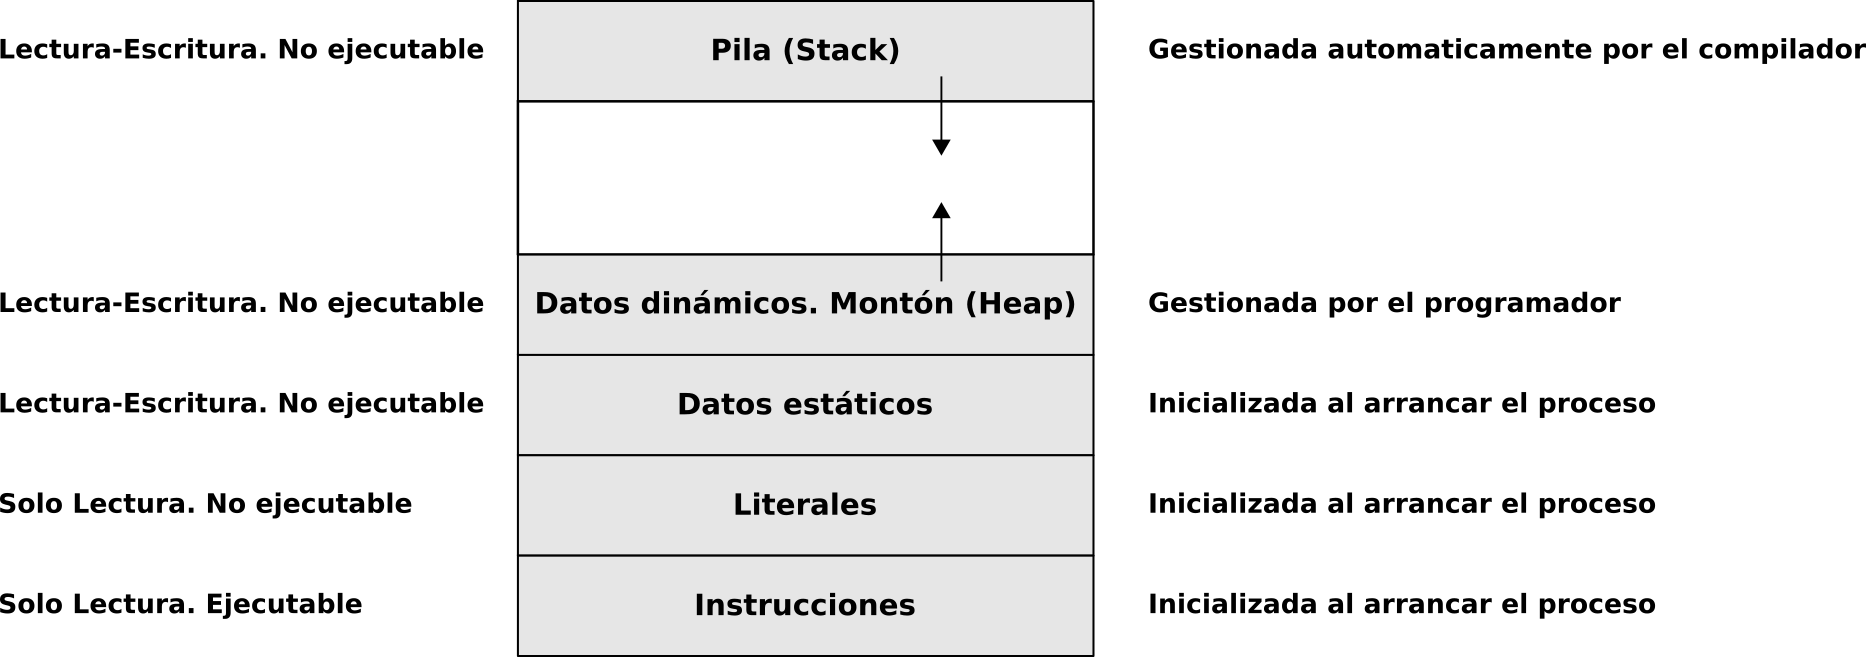
\includegraphics[width=0.75\linewidth]{img/memoria_segmentos.png}
	\caption{Segmentos de memoria durante la ejecución de un programa}
	\label{fig_segmentos_memoria}
\end{figure}

En programación, una \textit{variable} es un identificador (una etiqueta) que hace referencia a un determinado \textit{valor} almacenado en alguna posición de memoria. Es habitual referirse al valor utilizando el nombre de la variable, pero las \textit{variables} y los \textit{valores} a los que referencian son conceptos diferentes.

Durante la ejecución de los programas, las variables y sus datos asociados se guardan habitualmente en la memoria de pila (\textit{memoria stack}) o en la memoria \textit{heap}. Estos segmentos de memoria funcionan de manera diferente: la memoria \textit{stack} la gestiona el propio programa con un sistema LIFO (\textit{Last In First Out}), mientras que la memoria \textit{heap} necesita hacer llamadas al sistema operativo para asignar y liberar memoria. En general, el acceso y manipulación de los valores alojados en la memoria de pila es más rápido que el de la memoria \textit{heap}.

En Rust, la forma de almacenar en memoria los valores asociados a las variables depende del tipo de datos. En general, las variables de tipos de datos primitivos (enteros, coma flotante, bool y alguno más) guardan sus valores en la \textit{memoria de pila} (\textit{stack}). En cambio, las variables de otros tipos de datos, como las las cadenas de caracteres o los vectores, guardan sus valores en la \textit{memoria de montón} (heap). Estas variables, guardan en la pila un puntero a la posición de la memoria heap donde está el valor, además de algún metadato más de la variable.

Se podría decir que las variables cuyos valores son de tamaño conocido y constante en el momento de compilar se guardan en la memoria de pila y las variables de tamaño desconocido o que pueden variar de tamaño guardan sus valores en la memoria heap y sus metadatos en la pila. 

El código del Ejemplo \ref{ejstack1} muestra la declaración y asignación de valor a tres variables: un entero \textit{i32}, un valor en coma flotante \textit{f64} y un array con cinco valores enteros del tipo \textit{i32}. La función Rust \textit{std::mem::size\_of\_val()} devuelve el número de bytes ocupados en la memoria \textit{stack} por un valor determinado. Se puede comprobar que el número entero utiliza \textit{4} bytes para el almacenamiento, el \textit{f64} utiliza \textit{8} bytes y el array utiliza $5\times4=20$ bytes. Hay que tener en cuenta que, en Rust, los arrays tienen que definir su tamaño en tiempo de compilación y que dicho tamaño no se puede variar durante la ejecución del programa. Por ello, el tamaño total del array es conocido en tiempo de compilación y Rust guarda el valor del mismo en la memoria de pila.

\begin{EjemploCodigo}[Espacio de memoria ocupado por algunas variables]{ejstack1}
let n: i32 = 15;
println!("{}", std::mem::size_of_val(&n)); // Imprime 4
let x: f64 = 3.14;
println!("{}", std::mem::size_of_val(&x)); // Imprime 8
let v: [i32; 5] = [1, 2, 3, 4, 5];
println!("{}", std::mem::size_of_val(&v)); // Imprime 20
\end{EjemploCodigo}

Los tipos de datos cuyo tamaño no es conocido en tiempo de compilación o cuyo tamaño puede variar durante la ejecución del programa utilizan otra forma de almacenamiento. Lo que hace Rust es guardar en la pila (\textit{stack}) un puntero al lugar de la memoria \textit{heap} donde se guardará realmente el valor referenciado por la variable. Además, Rust puede guardar en la pila algún metadato más acerca de la variable. Por ejemplo, en el caso de las variables del tipo \textit{String} o \textit{Vec}\footnote{En realidad, internamente el tipo String es una estructura con un único campo del tipo Vec<u8>, un vector de bytes}, Rust guarda para cada variable el puntero a la memoria \textit{heap} que contiene el valor, el tamaño ocupado por el valor y la capacidad reservada en memoria para dicha variable, para que si aumenta de tamaño no haya que reasignar memoria a través del sistema operativo. La parte izquierda de la Figura \ref{fig_memoria_1} muestra un esquema del almacenamiento de una cadena de caracteres en memoria.

\begin{figure}[htb]
	\centering
	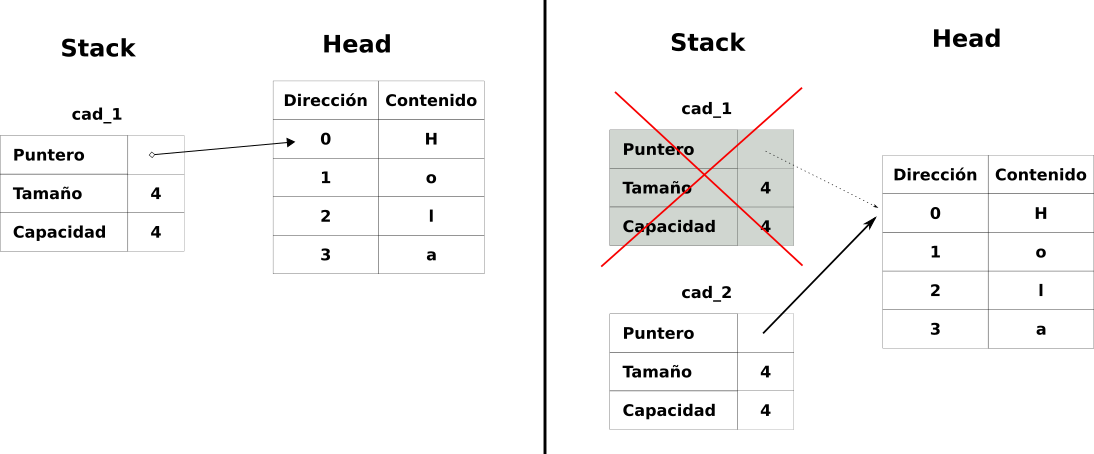
\includegraphics[width=0.9\linewidth]{img/memoria_1.png}
	\caption{Izq.: Almacenamiento en memoria de una variable del tipo \textit{String}. Dcha.: Tras asignar el valor de \textit{cad\_1} a la variable \textit{cad\_2}, la variable \textit{cad\_2} apunta al valor de la cadena y la variable \textit{cad\_1} deja de ser utilizable}
	\label{fig_memoria_1}
\end{figure}

\vspace{0em}
\begin{EjemploCodigo}[Almacenamiento en memoria de un String]{ejstring1}
fn main() {
   let s = String::from("Hola");
   println!("{}", std::mem::size_of_val(&s)); // Imprime 24=3x8
   println!("{}", s.len()); // Imprime 4, la longitud de la cadena
   println!("{}", s.capacity()); // Imprime 4, la capacidad de la cadena
   println!("{:p}", &s); // Imprime 0x7ffc8f9d9768, la dirección de s en la pila
   println!("{:p}", s.as_ptr()); // Imprime 0x625a2135eba0, la dirección de s en heap
}
\end{EjemploCodigo}

El código del Ejemplo \ref{ejstring1} crea una variable del tipo \textit{String} y le asigna un valor inicial. La función \textit{size\_of\_val()} devuelve \textit{24} bytes, que es el tamaño que ocupa una variable de cadena de caracteres en la memoria de pila. Los \textit{24} bytes corresponden a tres valores de \textit{8} bytes cada uno: la dirección de la memoria \textit{heap} en la que se guarda el \textit{String}, el tamaño de la cadena y la capacidad inicial de la cadena. Cada valor utiliza \textit{8} bytes porque ese es el tamaño del tipo de datos \textit{usize} que se utiliza en un procesador de \textit{64} bits para definir los punteros y los tamaños.

\begin{Nota}[Para saber más: \textit{Fat Pointers}]
Este tipo de almacenamiento en la pila (puntero más metadatos de la variable) suele recibir el nombre de \textit{fat pointer}.
\end{Nota}

Cuando se crea una variable y se le asigna un valor, dicho valor ocupa una parte de la memoria del programa. Los lenguajes de programación adoptan diferentes estrategias para decidir cuándo se puede liberar la memoria ocupada por un valor.

Hay lenguajes que utilizan un componente denominado \textit{Garbage Collector}, que se ejecuta periódicamente durante la ejecución del programa y libera la memoria de las variables que han dejado de ser utilizadas. La ejecución periódica del \textit{Garbage Collector} tiene varios efectos sobre los programas, entre otros, ralentizar la velocidad de ejecución y dar poco control al programador sobre la liberación de memoria. Este mecanismo es frecuente en lenguajes interpretados bien sean de \textit{tipado estático}, como Java, o de tipado dinámico, como Python.

\begin{Nota}[Para saber más: tipado estático Vs tipado dinámico]
	\small
	El \textit{tipado} de los lenguajes se refiere al momento en el que es necesario declarar el tipo de datos de las variables del programa. 
	
	En los lenguajes de \textit{tipado estático}, cualquier variable debe declarar el tipo de datos que va a guardar en el momento de la compilación. Es el caso de Java, C o Rust.
	
	En los lenguajes de \textit{tipado dinámico}, las variables pueden determinar  el tipo de datos que almacenan de manera dinámica, esto es, en tiempo de ejecución del programa. Así, una función se puede declarar con un parámetro genérico y utilizarla con argumentos de diferentes tipos de datos. Entre los lenguajes de tipado dinámico se encuentran Python o Javascript.
	
	En los lenguajes de tipado estático hay muchos errores de codificación que impiden la compilación del mismo y, por tanto, se detectan antes de la entrada en producción del programa. Por contra, en los lenguajes de tipado dinámico, hay errores que solo se detectan cuando el programa ya está en producción y que dificultan la realización de test y la depuración de los programas.
\end{Nota}
\vspace{1em}

Hay otros lenguajes, como C o C++, que descargan gran parte de la responsabilidad de la liberación de memoria en el programador. Al no ejecutarse el \textit{Garbage Collector}, ganan en velocidad de ejecución, aunque la dependencia del programador da lugar a importantes errores y problemas de seguridad de los programas.

Rust adopta un criterio diferente a los anteriores para gestionar la memoria, sin utilizar \textit{Garbage Collector} y estableciendo un criterio estricto acerca de la vida útil de los valores referenciados por las variables. El procedimiento utilizado por Rust se basa en el concepto que se ha denominado \textit{Propiedad de los Valores}.
 
La Propiedad de los valores afecta a las asignaciones y al paso de parámetros a funciones y otras construcciones de los programas. Se va a mostrar primero un ejemplo en Java de la asignación de unas variables a otras:

\begin{EjemploCodigo}[Ejemplo de asignación en Java]{ejjava1}
public class Prueba {
   public static void main(String[] args) {
      Point p1 = new Point(3,4);
      Point p2 = p1;
      p2.x = 10;
      System.out.println(p1.x); // Imprime 10
   }
}
class Point {
   int x;
   int y;	
   public Point(int x, int y) {
      this.x = x;
      this.y = y;
   }	
}
\end{EjemploCodigo}

En el código del Ejemplo \ref{ejjava1}, se crea una variable \textit{p1} del tipo \textit{Point} con valores \textit{(x=3, y=4)}. A continuación se crea una variable \textit{p2} y se le asigna el valor de la variable \textit{p1}. Se cambia el valor de la componente \textit{x} de \textit{p2}, dándole el valor \textit{10} y se imprime el valor de la componente \textit{x} de \textit{p1}, que resulta ser \textit{10}. ¿Que ha pasado?.

En Java, las variables del tipo objeto lo que guardan es una referencia al valor del objeto en memoria. Cuando se asigna un objeto a otro, no se crea un nuevo objeto, se copia la referencia, de forma que las dos variables quedan apuntando al mismo valor en memoria. En realidad hay un solo valor del objeto en memoria y dos referencias (las variables) apuntando al mismo objeto.


\section{Iteradores}

(Fuentes: 
\begin{itemize}
	\item \url{https://blog.jetbrains.com/rust/2024/03/12/rust-iterators-beyond-the-basics-part-i-building-blocks/})
	\item Module iter: \url{https://doc.rust-lang.org/std/iter/}
	\item Processing a Series of Items with Iterators: \url{https://doc.rust-lang.org/book/ch13-02-iterators.html}
\end{itemize}

Los iteradores son un patrón de diseño muy utilizado en la programación funcional y que se ha incorporado progresivamente en todos los lenguajes de programación. Su origen se marca en el lenguaje CLU del año 1973 \citep{wikipediaCLUProgrammingLanguage2024}.

Un \textit{Iterador} es un objeto que permite recorrer los elementos de una colección. Se suele hacer una distinción entre \textit{iteradores internos} y \textit{externos}. Los \textit{iteradores externos} serían objetos diferenciados de la propia colección que permiten recorrer uno a uno los elementos presentes en la colección. Los \textit{iteradores internos} serían más bien métodos o funciones proporcionados por la propia colección para realizar una tarea concreta sobre los elementos de la colección.

En Programación Orientada a Objetos, los iteradores internos se podrían equiparar con el patrón de diseño \textit{Visitor}, que definían de la siguiente manera The Gang of Four \citep{wikipediaDesignPatterns2024}:
 \begin{center}
	\begin{minipage}{0.9\linewidth}
		\vspace{5pt}%margen superior de minipage
		{\small \emph{Represent[ing] an operation to be performed on elements of an object structure. Visitor lets you define a new operation without changing the classes of the elements on which it operates.}
		}
		\vspace{5pt}%margen inferior de la minipage
	\end{minipage}
\end{center}

En Rust, los iteradores se basan en el trait \textit{Iterator}, que tiene la siguiente definición:

\vspace{0.7em}
\begin{Codigo2}
pub trait Iterator {
   type Item;
	
   fn next(&mut self) -> Option<Self::Item>;
	
   // Se omiten los métodos cuya implementación es automática
}
\end{Codigo2}

El trait está construido en base a dos elementos:

\begin{itemize}
	\item el método \textit{next()}, que permite determinar el siguiente elemento de una colección.
	\item el tipo de datos de los elementos que se van a recorrer, el \textit{type Item} que aparece en la definición del trait.
\end{itemize}

El trait no hace mención en ningún caso a la colección de objetos que se va a recorrer, lo que aumenta su flexibilidad. Los iteradores permiten definir funciones que describen la intención de lo que se quiere conseguir al procesar una fuente de datos, de manera independiente a la forma que adopten dichos datos. De esta forma, se podría cambiar la fuente de datos o su forma interna de organización, manteniendo las funciones que procesan dichos datos. Se trata de una codificación más declarativa que los bucles.

Para implementar el trait, hay que codificar el método \textit{next()}. El sistema se encarga de generar multitud de métodos de manera automática, como los métodos \textit{map()}, \textit{filter()}, o \textit{enumerate()}, por mencionar algunos de los más conocidos y que están presentes en la mayoría de los lenguajes de programación que disponen de iteradores. No obstante, en algunos casos puede  interesar sobrescribir alguno de estos métodos generados de manera automática, para conseguir una funcionalidad más ajustada a lo que se pretenda.

Realmente, lo que hacen estos métodos es crear un nuevo iterador a partir del iterador original. Se corresponderían con lo que se han denominado \textit{iteradores internos}, aunque también se suelen denominar \textit{adaptadores} (\textit{iterator adapters}). Es posible encadenar los métodos de forma que la salida de cada uno de estos métodos sea la entrada del siguiente, favoreciendo la \textit{canalización del procesamiento} de los datos (\textit{processing pipeline}). Una vez más, la codificación obtenida es declarativa y muestra de manera explícita qué se quiere hacer con los datos, en contra de lo que sucedería de realizar el mismo procesamiento a base de bucles.

Además de los métodos que se han denominado \textit{adaptadores}, el trait \textit{Iterator} genera de manera automática otros métodos que realizan directamente acciones sobre los elementos de la colección, como el método \textit{for\_each()}, que aplica una \textit{closure} a cada elemento, el método \textit{count()}, que cuenta los elementos existentes hasta el final del iterador, o el método \textit{collect()}, que reagrupa los elementos en una nueva estructura de datos en memoria.

Las colecciones que ofrece el lenguaje Rust permiten obtener un iterador sobre los elementos de la colección mediante el método \textit{into\_iter()}, o bien un iterador 
sobre referencias a los elementos de la colección utilizando el método \textit{iter()}.



\section{Razonamiento funcional de los programas}
Los programadores funcionales clasifican cualquier fragmento de código como acción, cálculo o datos. Esta clasificación puede recibir otras denominaciones, pero el concepto es el mismo. 

\begin{itemize}
	\item \textbf{Acciones:} son todo aquello que dependa de en qué momento se ejecuta o de cuántas veces se ejecuta. Por ejemplo, enviar un correo es una acción.
	\item \textbf{Cálculos:} son las tareas que solo dependen de los valores de entrada para generar un resultado. Los cálculos siempre devuelven el mismo resultado, si los valores de entrada son los mismos. Además, los cálculos nunca afectan a nada que esté fuera de ellos. Esto hace que los cálculos sean fáciles de testear y que su uso sea seguro, pues no hay que preocuparse de cuántas veces se utilicen o en qué orden sean invocados: si los parámetros de entrada son los mismos, el resultado será siempre el mismo.
	\item \textbf{Datos:} los datos son información registrada acerca de los acontecimientos. Tienen propiedades conocidas. Un mismo dato se puede interpretar de manera diferente según el contexto de ejecución en el que se encuadra. Por ejemplo, la factura de una cena la puede utilizar el cliente para llevar la cuenta de sus gastos mensuales o la puede utilizar el propietario del restaurante para determinar los gustos favoritos de sus clientes.
\end{itemize}

\begin{figure}[htb]
	\centering
	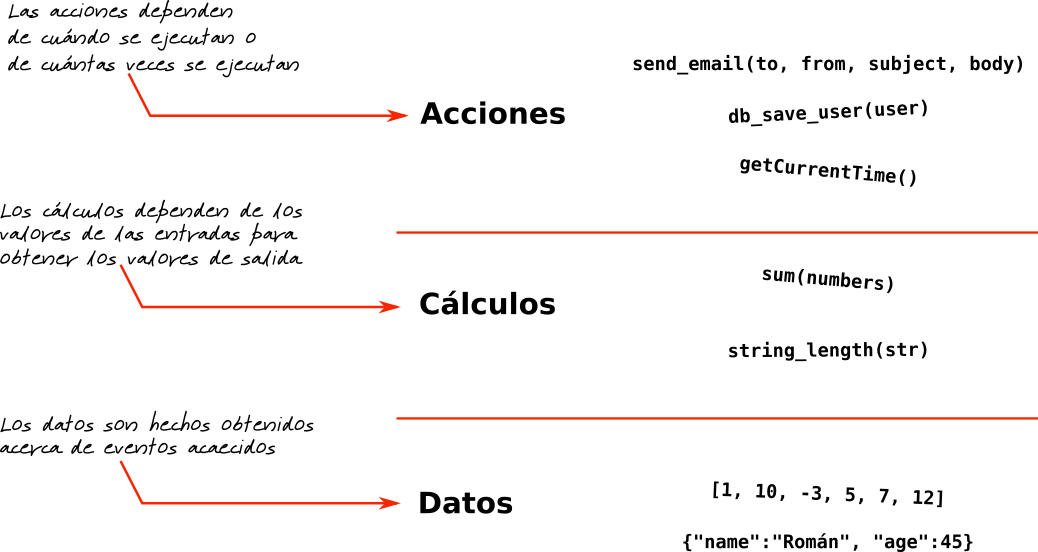
\includegraphics[width=0.9\linewidth]{img/AccCalcData.png}
	\caption{Ejemplos de código: Acciones, Cálculos y Datos}
	\label{fig_acccalcdata}
\end{figure}


La proliferación de los sistemas distribuidos en los que intervienen diferentes dispositivos y peticiones cuasi simultáneas de información a las bases de datos, el problema de organizar de manera adecuada el código se hace indispensable. En general, el código de las acciones será más difícil de comprender y de testear que el código de los cálculos, ya que estos últimos no dependen del número de veces que se invocan o del orden de dichas invocaciones. Es por ello que se hace importante separar en la medida de los posible el código que corresponde a las acciones del código que corresponde a los cálculos.

La programación funcional proporciona herramientas para el correcto tratamiento de cada una de estas categorías de código. En el caso de las acciones, es importante gestionar la forma en que cambia el estado de las variables del programa a lo largo del tiempo, garantizando el número de veces y el orden en el que se realiza cada acción. Los cálculos tienen su propia estrategia para comprobar su buen funcionamiento, a veces basada en técnicas matemáticas. En el caso de los datos, es importante organizarlos en estructuras que faciliten un acceso eficiente a la información que se quiere extraer de los mismos.
 
Hay dos técnicas fundamentales que permiten abordar los programas con un enfoque funcional: 
\begin{itemize}
	\item Distinguir en el código las acciones, de los cálculos y los datos.
	\item Utilizar abstracciones de primera clase.
\end{itemize}

A lo largo del curso se tratará de trasmitir el razonamiento funcional a la hora de abordar un problema de codificación. El objetivo es que las técnicas que se aprendan sean independientes del lenguaje que se utilice para programar y que sean de aplicación inmediata, tanto para la realización de un programa nuevo, como para refactorizar partes de un código ya existente.

Para clasificar el código en acciones, cálculos y datos es útil seguir los principios del \textit{diseño estratificado}, separando el código en diferentes capas. Para organizar el orden en el que se ejecutan las acciones son de utilidad los \textit{diagramas de tiempos} y la utilización de funciones de \textit{primera clase}, que permiten utilizar otras funciones como parámetros o resultados.

\subsection{Diseño estratificado}
En el diseño estratificado, se organiza el código en diferentes capas, ordenadas en función de la mayor o menor probabilidad de cambios en el código correspondiente a lo largo de la vida útil de la aplicación. Se suelen considerar tres capas principales:

\begin{itemize}
	\item \textbf{Nivel técnico:} correspondería a la parte de la aplicación que tiene menos probabilidades de cambiar. Por ejemplo, el lenguaje de programación de la aplicación o las estructuras de datos que se utilizarán para almacenar la información.
	\item \textbf{Reglas del dominio de la aplicación:} si por ejemplo se está haciendo una aplicación para gestionar unos cultivos de hortalizas, las distancia optima a la que hay que poner las plantas en el terreno o la cantidad de humedad que necesitan corresponden al campo de conocimiento de dicho dominio técnico y es difícil que cambien durante la vida útil de la aplicación.
	\item \textbf{Reglas del negocio:} se consideran aquí reglas que vienen marcadas por la aplicación concreta que se esté desarrollando. En el ejemplo de los cultivos podrían ser los precios de los factores de producción o la disponibilidad de determinados recursos.
\end{itemize}

Cada capa de la aplicación se desarrolla sobre las demás y solo debe depender de las capas que hay situadas por debajo de ella. De esta forma, si se produce una modificación en algún elemento, se sabe que solo puede afectar a los elementos que estén situados en la misma capa o en las capas superiores. La Figura \ref{fig_stratified} muestra un ejemplo de organización en capas de una aplicación para gestionar cultivos.

\vspace{1em}
\begin{figure}[htb]
	\centering \fbox{
		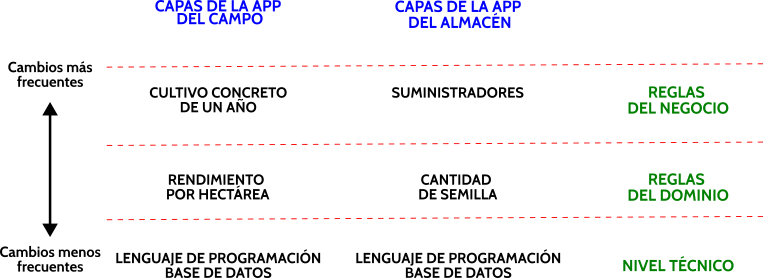
\includegraphics[width=0.8\textwidth]{img/stratified.png}
	}
	\caption{Esquema de capas en el diseño estratificado}
	\label{fig_stratified}
\end{figure}
 
\subsection{Líneas de tiempos}
En todas las aplicaciones hay que establecer el orden en el que se tienen que realizar las acciones. En aplicaciones sencillas, una distribución secuencial de las acciones puede ser suficiente. Pero, en sistemas distribuidos, en los que distintas tareas pueden correr a cargo de distintos componentes que pueden trabajar en paralelo o de forma concurrente, es importante establecer el orden en el que se tienen que realizar todas las acciones y los puntos en los que determinadas acciones no pueden ejecutarse si antes no se ha finalizado determinada acción anterior. Hay que cortar la línea de tiempos en algunos puntos para indicar que la ejecución no puede continuar hasta que se completen todas las tareas anteriores.

La Figura \ref{fig_timeline_1} muestra la línea de tiempos de una aplicación en la que, para poder ejecutarse las acciones \textit{D} y \textit{E} es necesario que primero se hayan completado las tareas llevadas a cabo por los componentes \textit{A}, \textit{B} y \textit{C}.

\vspace{1em}
\begin{figure}[htb]
	\centering \fbox{
		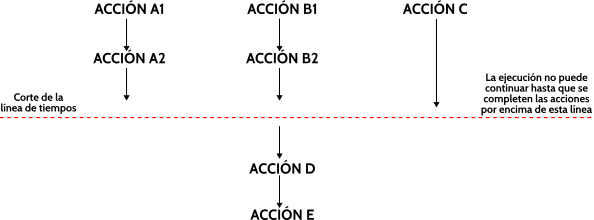
\includegraphics[width=0.65\textwidth]{img/timeline_1.png}
	}
	\caption{Cortando la línea de tiempo para garantizar el orden de ejecución de las acciones}
	\label{fig_timeline_1}
\end{figure}

La línea de tiempos ayuda a coordinar distintas acciones y a determinar los puntos en los que se pueden producir cuellos de botella durante la ejecución de los programas en sistemas distribuidos.

\section{Distinción entre acciones, cálculos y datos}
Antes de ponerse a codificar una aplicación nueva, conviene razonar .para distinguir qué elementos del programa serán acciones, cálculos o datos. En general, el orden de implementación consistirá en definir primero los datos, luego los cálculos y, por último, las acciones.

Cuando se está analizando un código ya existente, habrá que identificar igualmente las funciones que incluyen acciones. En muchos casos, una misma función incluirá acciones y cálculos. En esos casos, conviene refactorizar para separar las acciones de los cálculos.  

Como se ha comentado, las acciones dependen de cuándo se ejecutan o de cuantas veces se ejecutan. Las funciones que implementan acciones se suelen denominar \textit{funciones impuras} o \textit{funciones con efectos secundarios}. Enviar un correo o leer datos de una base de datos serían ejemplos de acciones.

Por el contrario, los cálculos solo dependen del valor de los parámetros de entrada y no producen efectos secundarios. Se denominan \textit{funciones puras} o \textit{funciones matemáticas}. Calcular el máximo de una serie de números o comprobar si determinada dirección de correo es válida podrían ser ejemplos de funciones puras. 

Se dice que los cálculos son \textit{referencialmente trasparentes}. La trasparencia referencial significa que se puede sustituir el cálculo por el resultado sin que el programa se vea afectado. Por ejemplo, si una función realiza la suma de dos números, en los lugares del programa donde se hace la llamada a la función se puede sustituir ésta por el resultado de la suma y el programa no se verá afectado.

Los datos son hechos.

\subsection{Entradas y salidas implícitas}
Los parámetros de una función son el procedimiento de \textit{entrada explícita} de datos a la función. El valor devuelto por la función es la salida \textit{explícita}. 
Cuando una función es impura, tiene entradas o salidas implícitas. Se denomina \textit{entrada implícita} a la entrada de datos a la función que no procede de un parámetro. Se denomina \textit{salida implícita} al valor que sale de la función sin hacerlo a través del valor devuelto por la misma.

El código del ejemplo muestra una función denominada \textit{contador\_impuro()} que no tiene parámetros ni devuelve ningún valor. En cambio, la función recibe como entrada implícita el valor de un contador existente en la base de datos, a través de un método llamado \textit{get\_contador\_from\_database()}, y realiza una salida también implícita reescribiendo en la base de datos el valor incrementado de dicho contador a través del método \textit{update\_contador\_in\_database()}. La salida implícita de la función es, además, un efecto secundario de la misma, convirtiendo a dicha función en una \textit{acción}.

\begin{EjemploCodigo}[Entradas y salidas implícitas]{ejimplicita1}
fn contador_impuro() {
   let contador = get_contador_from_database(); // Entrada implícita
   update_contador_in_database(contador+1); // Salida implícita
}
\end{EjemploCodigo}

El acceso a variables globales dentro de una función es una forma de entrada o salida implícita.

En la medida de lo posible, hay que evitar las entradas y salidas implícitas, pues complican la trazabilidad y la facilidad de testeo de las funciones. En muchas ocasiones, las entradas implícitas se pueden sustituir por parámetros de la función. De la misma forma, las salidas implícitas es posible sustituirlas por valores devueltos por las funciones.


\section{Ejemplo}

\begin{EjemploCodigo}[Ejemplo carrito]{}
struct Producto {
   name: String,
   precio: f64,
}
fn main() {
   let mut carrito = Vec::<Producto>::new();
   let mut total_compra: f64 = 0.0;
   let producto = Producto{name: "Sandalias".to_string(), precio: 12.5};
   add_producto(producto, &mut carrito, &mut total_compra);
}
fn add_producto(producto: Producto, carrito: &mut Vec<Producto>, total_compra: &mut f64) {
   carrito.push(producto);
   calc_total_carrito(carrito, total_compra);
}
fn calc_total_carrito(carrito: &mut Carrito, total_compra: &mut f64) {
   *total_compra = 0.0;
   for producto in &carrito.items {
      *total_compra = *total_compra + producto.precio;
   }
   actualiza_web_total_compra( *total_compra);	
}
fn actualiza_web_total_compra(total_compra: f64) {  }
\end{EjemploCodigo}


%\begin{EjemploCodigo}[]{}
%\end{EjemploCodigo}

%
%
%\begin{EjemploCodigo}[]{}
%	
%\end{EjemploCodigo}

  
\section{Functional Programming made easier (Scalfani)}

\section{1.- Discipline is freedom}
\subsection{Global State}
El uso de varibles globales conlleva determinados inconvenientes:
\begin{itemize}
	\item Cualquiera desde cualquier módulo puede cambiar el valor de las variables globales.
	\item Se producen acoplamientos de las variables globales entre sí y de unos módulos con otros.
	\item En programación concurrente no hay garantías respecto de la modificación de las variables.
	\item Colisión de nombres entre las variables globales y otros identificadores en cualquier módulo.
\end{itemize}

En el caso de la programación orientada a objetos se produce la misma circunstancia con el patrón \textit{Singleton}.

Los lenguajes de PF prohíben la existencia de variables globales. Rust permite solo la existencia de constantes globales.

\subsection{Mutable State}
La posibilidad de que las variables puedan cambiar de valor también tiene algunos inconvenientes. Por ejemplo, es más difícil razonar sobre el código, pues los valores que pueden cambiar pueden hacer cambiar también la semántica del programa, o hacer el código más frágil.

En los lenguajes funcionales, las variables son inmutables y ello da lugar a algunas consecuencias.
\begin{itemize}
	\item Las expresiones del tipo $x = x +1$ no tienen sentido. Una vez que se asigna un valor a $x$, no se puede cambiar.
	\item Las asignaciones como $x=20$ son \textit{expresiones referencialmente trasparentes}, esto es, en cualquier parte del programa se puede utilizar indistintamente $x$ o $20$ con la seguridad de que el programa seguirá funcionando igual. La trasparencia referencial permite una evaluación \textit{lazy} de la sustitución de $x$ por su valor en el código.
\end{itemize}

Si las variables no pueden cambiar de estado, no es posible hacer bucles. En los lenguajes funcionales, los bucles se sustituyen por la recursividad. Cualquier bucle se puede ejecutar mediante recursividad y viceversa.

Por ejemplo, la definición matemática del factorial de un número se podría hacer de la siguiente forma:
\begin{equation}
\label{eq_factorial_1}
n! = 1.2...(n-2).(n-1).n \quad \forall n \in \mathds{N} 	
\end{equation}
Con esta definición, parecería inmediato resolver el problema con un bucle, como se hace en el Ejemplo \ref{ejfactorial1}.

\vspace{1em}
\begin{EjemploCodigo}[Factorial calculado con un bucle]{ejfactorial1}
fn factorial_bucle(n: u32) -> u32 {
   let mut prod = 1;
      for i in 1..=n {
         prod = prod*i;
      }
   prod
}
\end{EjemploCodigo}

Si en la Expresión \ref{eq_factorial_1} se cambia el orden del producto, los términos se podrían agrupar de la siguiente manera:
\begin{equation}
\label{eq_factorial_2}
n! = n.(n-1)...2.1 \quad = n . (n-1)! \quad \forall n \in \mathds{N} 	
\end{equation}

Con esta definición surge el problema de calcular $0!$, pero su valor se puede deducir. De la Expresión \ref{eq_factorial_1} se sabe que $!1 = 1$. Se podría operar de la siguiente forma:
\begin{align*}
1! &= 1 \\
1! &= 1. (1-1)! = 1 . 0! \\
1  &= 1 . 0! = 0! \\
\end{align*}

Con lo que finalmente queda que:
\begin{equation}
\label{eq_factorial_3}
0! = 1
\end{equation}
Una vez calculado el valor de $0!$, se puede proceder a definir el factorial de cualquier número natural con la siguiente definición recursiva:
\begin{align} \label{eq_factorial_4}		
0! &= 1 \nonumber \\
n! &= n . (n-1)! \quad \forall n \in \mathds{N} 
\end{align}

Esta definición de factorial se podría codificar como se hace en el Ejemplo \ref{ejfactorial2}.

\vspace{1em}
\begin{EjemploCodigo}[Factorial calculado de manera recursiva]{ejfactorial2}
fn factorial_recursivo(n: u32) -> u32 {
   match n {
      0 => 1,
      _ => n*factorial_recursivo(n-1)
   }
}
\end{EjemploCodigo}



\section{Variables globales}

{\small\color{blue}(Apuntes tomados del artículo: de Jakob Meier titulado <<How to Idiomatically Use Global Variables in Rust>> \citep{meierHowIdiomaticallyUse2021})}

Vamos a ver en primer lugar cómo no se pueden usar las variables globales en Rust. Podríamos estar tentados de usar sentencias \textit{let}, como en la variables locales de cualquier función:

\vspace{0.7em}
\begin{Codigo2}
use chrono::Utc;

let START_TIME: String = Utc::now().to_string();

fn main() {
   ...
}
\end{Codigo2}

El código anterior no compila, no se pueden usar asignaciones \textit{let} en el ámbito global, pues la instrucción \textit{let} crea una variable en la memoria stack, que no se inicializa hasta que se ejecuta el programa. Las variables globales solo se pueden crear utilizando las cláusulas \textit{const} o \textit{static}, que utilizan la memoria del segmento de datos (\textit{data segment}) del programa. 

Tampoco se puede compilar la siguiente inicialización:

\vspace{0.7em}
\begin{Codigo2}
use chrono::Utc;

static START_TIME: String = Utc::now().to_string();
	
fn main() {
   ...
}
\end{Codigo2}

El compilador avisa que no se pueden utilizar funciones no constantes en la inicialización de variables globales. No se puede ejecutar ningún tipo de código antes de que el programa comience. El valor de una variable global debe ser conocido en el momento de la compilación, antes de la ejecución. 

Tampoco valdría declarar la variable global y tratar de asignarle valor en \textit{main()}:

\vspace{0.7em}
\begin{Codigo2}
use chrono::Utc;

static START_TIME: String;

pub fn main() {
   START_TIME =  = Utc::now().to_string();
   println!("{}", START_TIME);
}
\end{Codigo2}

El código anterior tampoco compila, el compilador nos avisa de que hay que asignar algún valor a la variable \textit{static}. Podríamos pensar en asignarle un valor \textit{None}

\vspace{0.7em}
\begin{Codigo2}
use chrono::Utc;

static mut START_TIME: Option<String> = None;

pub fn main() {
   START_TIME = Some(Utc::now().to_string());
   println!("{}", START_TIME);
}	
\end{Codigo2}

Pero el código anterior tampoco compila, el compilador nos avisa de que una variable global mutable solo se puede utilizar dentro de un bloque inseguro \textit{unsafe{}}. Finalmente, si encerramos el código dentro de \textit{main()} en un bloque \textit{unsafe{}}, sí que compila:

\begin{Codigo2}
use chrono::Utc;

static mut START_TIME: Option<String> = None;

pub fn main() {
   unsafe{
      START_TIME =  Some(Utc::now().to_string());
      println!("{}",  START_TIME.clone().unwrap());
   };
}
\end{Codigo2}

Ahora, el código compila y se puede ejecutar, pero no parece una forma muy cómoda de utilizar, aunque en algunas ocasiones pudiera ser útil.

Vamos a ver otro problema relacionado con la extensión del dominio de las variables. En un programa como el anterior, no se necesitaría declarar la variable como global, se podría declarar dentro de la función \textit{main()}. Pero suponga que lo que se quiere es utilizar la variable en un hilo diferente creado dentro de \textit{main()}

\begin{Codigo2}
use chrono::Utc;

pub fn main() {
   let start_time = Utc::now().to_string();
   
   let thread_1 = std::thread::spawn(||{
      println!("Started {}, called thread 1 {}", &start_time, Utc::now());
   });
	
   thread_1.join().unwrap();
}
\end{Codigo2}

Si tratamos de compilar este código, el compilador nos dirá que el hilo \textit{thread\_1} podría vivir más tiempo que la variable \textit{start\_time} que se ha creado en el marco de datos en el stack de la función \textit{main()} y no está garantizado que la variable sobreviva lo suficiente. Nosotros, viendo el código, sabemos que al hacer el \textit{join()} antes de salir de \textit{main()} estamos garantizando esa supervivencia, pero el compilador no nos deja compartir con otros hilos variables que no tengan una vida útil \textit{\&static}.

Hay un par de soluciones posibles sin utilizar variables globales. La primera sería clonar la variable \textit{start\_time} y pasar a la closure la propiedad del valor clonado:

\begin{Codigo2}
pub fn main() {
   let start_time = Utc::now().to_string();
   let cloned_start_time = start_time.clone();
   let thread_1 = std::thread::spawn( move ||{
      println!("Started {}, called thread 1 {}", &cloned_start_time, Utc::now());
   });
   thread_1.join().unwrap();
}	
\end{Codigo2}

Esta solución puede servir para una variable de cadena de caracteres como la anterior, pero si hubiera que clonar una variable de mayor tamaño podría no ser la solución óptima. En esos casos se podría envolver la variable con un puntero \textit{Arc}:



\begin{Codigo2}
use chrono::Utc;
use std::sync::Arc;

pub fn main() {
   let start_time = Arc::new(Utc::now().to_string());
   let cloned_start_time = Arc::clone(&start_time);
   let thread_1 = std::thread::spawn(move ||{
      println!("Started {}, called thread 1 {}", &cloned_start_time, Utc::now());
   });
	
   thread_1.join().unwrap();
}
\end{Codigo2}

Si además se necesitara mutabilidad interior de la variable, se podría envolver en un \verb+ Arc<Mutex<String>>+.

\subsection{Valor conocido en tiempo de compilación}
Cuando el valor de la variable global se conoce en tiempo de compilación, hay básicamente dos soluciones:
\begin{itemize}
	\item \textbf{const:} valores constantes que se conocen en tiempo de compilación. No permiten la mutabilidad interior. El compilador resuelve sustituyendo el valor en línea (inline)\footnote{Conviene consultar el apartado de la cláusula \textit{const} en la documentación en  \url{https://doc.rust-lang.org/std/keyword.const.html} y del concepto de \textit{expresiones constantes} en \url{https://doc.rust-lang.org/reference/const_eval.html}}. 
	\item \textbf{static:} las variables reciben un espacio de memoria en el segmento de datos. Es posible la mutabilidad interior.
\end{itemize}

Si se necesita mutabilidad interior, para los tipos primitivos se pueden utilizar valores \textit{atomic} \footnote{Ver libro en líne de Mara Bos \url{https://marabos.nl/atomics/}} y, para tipos más complejos, se pueden usar \textit{locks} en la forma \textit{read-write lock}, \textit{RwLock} o en la forma \textit{mutual exclusion lock}, \textit{Mutex}. 

Si lo que se necesita es calcular el valor en tiempo de ejecución, las soluciones con \textit{const} y \textit{static} no sirven.

{\color{blue}(No he terminado de sacar los apuntes del artículo)}

\pagebreak
\bibliography{Mibiblioteca}



\end{document}


